\documentclass[11pt,a4paper]{article}
\usepackage[utf8]{inputenc}
\usepackage[german]{babel}
\usepackage{amsmath}
\usepackage{amsfonts}
\usepackage{amssymb}
\usepackage{graphicx}
\usepackage[left=2cm,right=2cm,top=2cm,bottom=2cm]{geometry}

\author{AlphaNerd}
\title{Systeme Wissensfragen}

\begin{document}
\maketitle


\subsection*{Kapitel 2: Überblick}
\begin{itemize}
\item[1)]
Verschiedene Arten von Betriebssystemen werden für verschiedene Verwendungszwecke benutzt. Nennen sie 4 Arten von Betriebssystemen.
\end{itemize}


\subsection*{Kaptiel 3: Dateisytseme}
\begin{itemize}
\item[1)] Nennen sie 5 Dateiattribute (Metadaten) die vom Betriebssystem angelegt werden.
\item[2)] Wie unterscheiden sich die rwx Rechte für Dateien und Verzeichnisse?
\item[3)] Welche Auswirkung hat das setzen des SUID- bzw. SGID-Flags auf die Dateirechteverteilung?
\item[4)] Wie verhalten sich mit \texttt{ln -s QUELLE ZIEL} erstellte Dateien im Vergleich zu mit \texttt{ln QUELLE ZIEL} erstellte Dateien? Sind Verzeichnisse als \texttt{QUELLE} gültig?
\item[5)] Geben sie die minimale Zugriffszeit auf das n-te Byte bei a) Sequentiellen Speichertypen und b) Random-Access-Memory an.
\item[6)] Geben sie 6 Systemaufrufe (Operationen) auf a) Dateien und b) Verzeichnisse an.
\item[7)] Welche Vor- und Nachteile besitzt die Realisierung von Dateien als zusammenhängende Belegung (2 Nennungen)? Wo wird diese eingesetzt?
\item[8)] Welche Vor- und Nachteile besitzt die Realisierung von Dateien als verkettete Listen auf der Festplatte (3 Nennungen)? Wie verändern sich diese beim benutzen einer FAT?
\item[9)] Welchen Einfluss hat die Wahl der Blockgröße auf die Performance eines Fat32 Dateisystems?
\item[10)] RAID 0: Striping \\RAID 1: Mirroring \\ RAID 5: Block-Level Striping mit verteilter Parität.\\
\\
Skizzieren sie die Realisierung von RAID 0/1/5.
\end{itemize}


\subsection*{Kapitel 4: Prozesse}
\begin{itemize}
\item[1)] Erklären sie den Unterschied zwischen Programm, Prozess und Threads. Welche Informationen werden jeweils verwaltet (jeweils 3 Nennungen).
\item[2)] Wie funktioniert Pseudoparallelität?
\item[3)] Zeichnen sie ein Zustandsdiagramm für Prozesse mit Nichtpräemptivem und prämptivem Scheduling, mit und ohne Auslagerung.
\end{itemize}


\pagebreak


\subsection*{Kapitel 5: Nebenläufigkeit}
\begin{itemize}
\item[1)] Erläutern sie den Bergriff \glqq Racecondition\grqq.
\item[2)] Nennen sie die 4 Anforderungen an Lösungen für das Problem der kritischen Region.
\item[3)] Wie wollen die Tutoren umbedingt einen Widerspruchsbeweis strukturiert haben?
\item[4)] Beweisen sie, dass durch diese Implementierung ein wechselseitiger Ausschluss garntiert ist. Welcher Nachteil ergibt sich durch diese Realisierung?\\
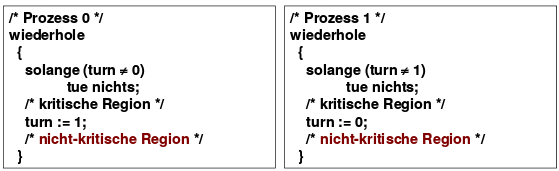
\includegraphics[scale=0.7]{kap5strikt.png}
\item[5)] Nennen sie den Nachteil von reinen Softwarelösungen für die Lösung für das Problem der kritischen Region.
\item[6)] Nennen und erklären sie einen der Assembler Befehle der für eine atomare Ausführung sorgt.
\item[7)] Welchen Nachteil birgt eine reine Hardwarelösung?
\item[8)] Welche Daten (3) und Operationen (2) besitzt ein Mutex?
\item[9)] Welche Situation beschreibt a) \texttt{$count_s < 0$} \ \ \ b) \texttt{$count_s = 0$} \ \ und \ c)  \texttt{$count_s > 0$} bei einer Semaphore s?
\item[10)] Implementieren sie eine Lösung für das Produzenten-Konsumenten-Problem für 2 Produzenten, 2 Konsumenten und einer Buffergröße von n, der Buffer sei Anfangs leer. Achten sie auf die Initialisierung ihrer Semaphoren.
\end{itemize}


\subsection*{Kapitel 6: Deadlocks}
\begin{itemize}
\item[1)] Welche 4 Vorraussetzungen müssen für das Auftreten von Deadlocks gegeben sein?
\item[2)] Wann existiert immer eine Ausführungsreihenfolge die zu keinem Deadlock führt?
\item[3)] Welche Vorraussetzungen benötigt der Bankieralgorithmus um eine Deadlock freie Ausführungsreihenfolge zu garantieren (2)?
\item[4)] Warum existiert für manche vom Bankieralgorithmus als unsicher eingestufte Ausführungen trotzdem eine Deadlock freie Restausführung (2 Nennungen)?
\item[5)] Welche Matrizen benötigt der Bankieralgorithmus?
\item[6)] Warum ist durch den Bankieralgorithmus das Deadlockproblem nicht restlos gelöst (3 Nennungen)?
\item[7)] Welche Bewältigungsstrategien gibt es für die Behebung von Deadlocks (2 Nennungen)?
\end{itemize}


\pagebreak


\subsection*{Kapitel 7: Scheduling}
\begin{itemize}
\item[1)] Nennen und beschreiben sie die 3 Arten von Scheduling.
\item[2)] Worin liegt der Unterschied zwischen Benutzer- und Systemorientiertem Scheduling (3 Nennungen)?
\item[3)] Bestimmen sie die Auswahlfunktion, sowie die Zuordnung zu nicht- beziehungsweise präemptivem Scheduling von folgenden Strategien:
\begin{enumerate}
\item First Come First Served (FCFS)
\item Round Robin (RR)
\item Shortest Job First (SJF)
\item Shortest Remaining Time (SRT)
\item Highest Response Ratio Next (HRRN)
\end{enumerate}
\item[4)] Erläutern sie kurz Feedback beziehungsweise Unixscheduling.
\item[5)] Analysieren sie die Schedulingstrategien aus Aufgabe 3 in Hinsicht auf a) Bevorzugung von kurzen/langen Prozessen, b) Livelock Gefahr, c) eventuellen Wissensanforderungen und d) Effektivität im Sinne der Benutzer- beziehungsweise Systemorientierter Anwendung.
\end{itemize}


\subsection*{Kapitel 8: Speicherverwaltung}
\begin{itemize}
\item[1)] Skizzieren sie die Speicherhierache (5 Nennungen).
\item[2)] Welche 5 Anforderungen werden an die Speicherverwaltung gestellt? Erläutern sie diese kurz.
\item[3)] Wie stehen physikalische, logische und relative Adressen im Zusammenhang?
\item[4)] Wie können Namensräume von Prozessen vor einander geschützt werden? Skizzieren sie.
\item[5)] Welche Vor- und Nachteile treten bei den drei Varianten der Partitionierung auf? (Jeweils 3, 3 und 1 Nennungen.
\item[6)] Nennen sie die drei Speicherzuteilungsalgorithmen, welcher ist am effektivsten? Welche Nebeneffekte treten bei den anderen beiden auf?
\item[7)] Welche Größe muss das Offset-Feld beim einfachen Paging mindestens haben, wenn die Seitengröße $2^{11}$ Bit beträgt?
\item[8)] Erklären sie den Begriff des virtuellen Speichers. Welche Vor- und Nachteile ergeben sich dadurch (jew. 2 Nennungen)? Durch welches Prinzip ist die Verwendung trotzdem sinnvoll? Was würde ohne dieses Prinzip passieren? 
\item[9)] Welche Einträge besitzt die Seitentabelle bei Paging mit virtuellem Speicher?
\item[10)] Skizzieren sie die Adressumsetzung für Paging mit virtuellem Speicher.
\item[11)] Beschreiben sie kurz das Prinzip der mehrstufigen Seitentabellen.
\item[12)] Beschreiben sie kurz das Prinzip der invertierten Seitentabellen, gehen sie dabei auch auf die Adressumsetzung ein.
\item[13)] Beschreiben sie die Grundidee der Speicherverwaltung durch Segmentierung.
\item[14)] Nennen sie 2 Austauschstrategien.
\end{itemize}


\pagebreak


\subsection*{Kapitel 9: Sicherheit}
\begin{itemize}
\item[1)] Worin besteht der Unterschied zwischen Betriebs- und Angriffssicherheit?
\item[2)] Nennen sie die 4 Sicherheitsziele.
\item[3)] Nennen sie 2 Verschlüsselungsstrategien.
\end{itemize}











\end{document}